\documentclass{article}
\usepackage{graphicx}
\usepackage{amsmath}
\usepackage{graphicx}
\usepackage{fancyhdr}
\usepackage{amsfonts}
\usepackage{float}
\DeclareGraphicsExtensions{.png}


\title{COSC264 Assignment 1}
\author{Dillon Thorsteinn George 38063248 Carl Kenny 93678486}
\date{}

\pagestyle{fancy}
\lhead{Dillon George 38063248}
\rhead{Carl Kenny 93678486}

\begin{document}

\maketitle{}
\null  % Empty line
\nointerlineskip  % No skip for prev line
\vfill
\let\snewpage \newpage
\let\newpage \relax
\let \newpage \snewpage
\vfill 
\break % page break

\newpage

\section*{Question 1}
Binomial distribution was used to compute the number of successful trials in n independent experiments.
Each bit's error rate is independent of other bits. An assumption has been made that the
head of the packet will be error-free, hence errors may only appear in the user-data. The
coefficient was calculated using Python's scipy module.

\section*{Question 2}
The distribution of packet errors follows a binomial model. The probabilty of having $m$
bit errors in a message of length $n$ is:
\[
        P(X=m) = {n\choose m} p^m (1-p)^{n-m}
\]
Where $p$ is the probabilty of a bit error.
The probabilty of having atleast one bit error is thus:
\begin{align*}
        P(X\geq 1) &= 1 - P(X = 0) \\
                   &= 1 - {n\choose 0} p^0 (1-p)^{n} \\
                   &= 1 - (1 - p)^{n}
\end{align*}

\section*{Question 3}
\begin{figure}[H]
    \centering
    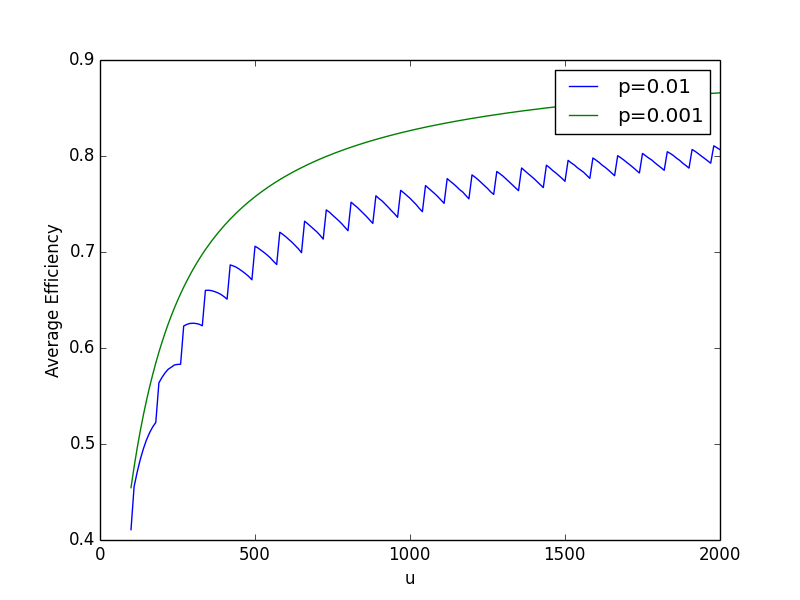
\includegraphics[width=0.8\textwidth]{q3.png}
    \caption{Awesome Image}
    \label{fig:awesome_image}
\end{figure}



\section*{Question 4}
The user data (u) was set as 512. As the bit error probability increased, the average number of retransmissions increases consequently and efficiency falls proportionately.
\begin{figure}[H]
    \centering
    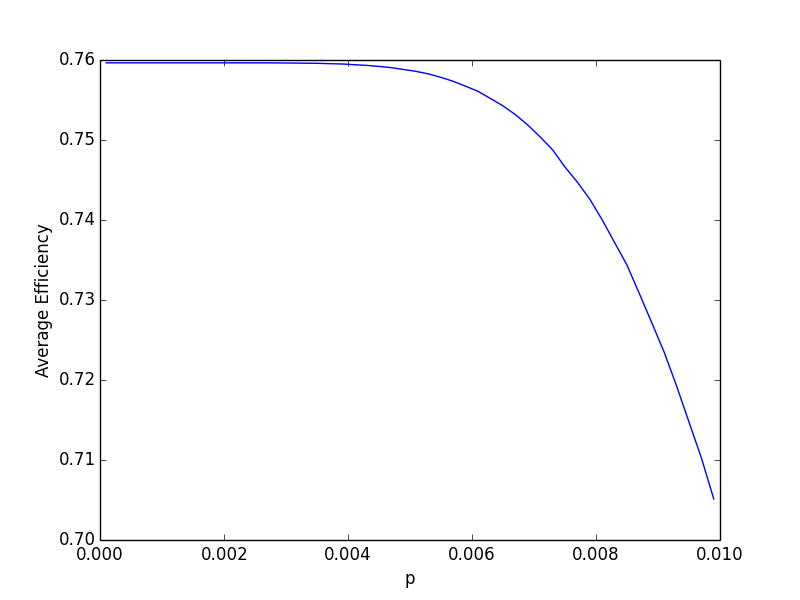
\includegraphics[width=0.8\textwidth]{q4.png}
    \caption{Awesome Image}
    \label{fig:awesome_image}
\end{figure}



\section*{Question 5}
 The two-state channel is an attempt to replicate 'bursty' network conditions. Time is split per packet transmission or retransmissions, with the state of the channel being determined by the previous channel state and a fresh uniform random number, q. The uniform random number is generated via the numpy module, specifically using random.uniform()

The two-state channel switches between two states. The 'good-state' has a bit error probability of 10E-5 where as the 'bad-state' has a bit error probability set as 1.99*10E-3. Importantly, this leads to a long-term average of 10E-3. Errors while the channel is in a good-state are very unlikely, hence the bad-state contributes more heavily towards retransmissions.

The initial drop in efficiency is like due to the small number of checkbits and an unlucky set of trials. Two-state channel's average efficiency rises towards a threshold where it unites with the BSC channel. <insert calculation of said threshold> As displayed by the plot, once the two-state channel reaches the threshold it shares the same average efficiency as the BSC channel.


\begin{figure}[H]
    \centering
    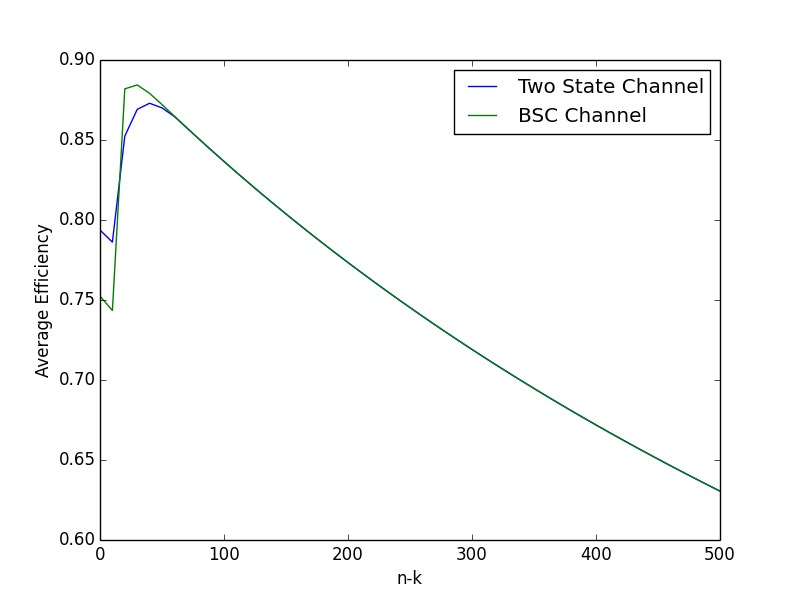
\includegraphics[width=0.8\textwidth]{q5.png}
    \caption{Awesome Image}
    \label{fig:awesome_image}
\end{figure}

\end{document}
